\scanpage{16}
Polygône régulier (ou réalisation régulière d'un polygône combinatoire) : définitions possibles (cotés égaux, angles égaux, \tikz[baseline=(trans.base)]{
\node[anchor=base west,inner sep=0pt] (trans) at (0,0) {transitivité};
\node[anchor=base west,inner sep=0pt] at (-.75,.62) {\inserted{\deleted{\unsure{il suffit|il faut|il y avait}} les deux,}};
\draw (-.36,-.20) .. controls (-.36,.30) and (-.15,.43) .. (.20,.43)
 -- (3.20,.36) .. controls (3.37,.36) and (3.47,.39) .. (3.50,.47);
} groupe des symétries ...) Existence, unicité modulo homothétie :
\reversemarginpar
\margin{\figure{\begin{tikzpicture}[x=.8cm,y=.8cm]
\draw (0,0) -- (1.12,.65);
\draw (1.16,.73) -- (1.54,1.91);
% A detached triangular trace: writing versus surface trace remains uncertain.
\node[inner sep=0pt] at (.66,1.19) {\unsure{\tikz[baseline=0pt]{\fill (0,0) -- (.025,.055) -- (.055,.015) -- cycle;}}};
\end{tikzpicture}}}
\normalmarginpar
tout isom. combinatoire est induit par une unique similitude.

Notion d'enveloppe affine (ou vectorielle) d'un polygône combinatoire ... \unsure{sens|sen.|sans} précisé

\noindent
\begin{tikzpicture}[x=1cm,y=1cm,baseline=(fun.base)]
\node[anchor=base west,inner sep=0pt] (fun) at (0,0) {Fonctorialité de $X\times_G Y$ p.r. \unsure{à|:} $(\unsure{G|X},X,Y)$ ...};
% The two separate rules surround part of the line; neither underlines its opening word.
\draw (3.58,.40) -- (6.66,.40);
\draw (3.48,-.24) .. controls (4.70,-.35) and (6.02,-.28) .. (7.00,-.23);
\end{tikzpicture}

\[
\begin{aligned}
\unsure{P|\overline{P}}\times_G E={}^{P}\!\deleted{B}E=F
&\qquad\qquad &P&\quad G\text{-torseur}\\
&&E&\quad G\text{-ensemble}
\end{aligned}
\]

$P\longrightarrow\operatorname{Bij}(E,F)$ compatible aux opérations de $G$ à droite

\uline{NB} Si $G$ opère fidèlement sur $E$, $G$ opère ``sans pts fixes'' sur $\operatorname{Bij}(E,F)$ --- i.e. $\deleted{\unsure{y}}\unsure{x|y}.g=\unsure{x|u}$ $(g\in G,\ x\in B)$ implique $g=1$, ou encore les $G_{\unsure{u|x}}$ $(u\in B)$ sont réduits à $\{1\}$, ou encore $B$ est une somme de torseurs ... Dans ce \tikz[baseline=(cas.base)]{
\node[anchor=base west,inner sep=0pt] (cas) at (0,0) {cas,};
\node[anchor=base west,inner sep=0pt] at (1.00,0) {$P\mathbin{\text{---}}\operatorname{Bij}(E,F)$ est injectif};
\node[anchor=base west,inner sep=0pt] at (.08,.62) {\inserted{et dans ce cas seulement}};
\draw (.47,-.30) .. controls (.60,.42) and (.87,.45) .. (1.35,.45)
 .. controls (2.80,.51) and (4.60,.31) .. (5.12,.43);
}

\[
P\hookrightarrow\operatorname{Bij}(E,F)
\]

\reversemarginpar
% slanted: the two-line note rises towards the right, above its brace.
\margin{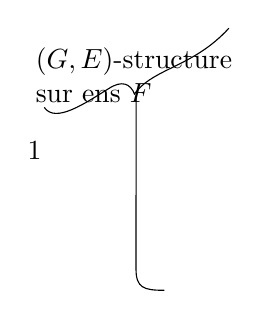
\begin{tikzpicture}[x=1cm,y=1cm,baseline=(ref.base)]
\node[inner sep=0pt] (ref) at (0,0) {};
\begin{scope}[shift={(-.48,1.20)},rotate=25]
\node[anchor=south west,inner sep=0pt] at (0,0) {\shortstack[l]{$(G,E)$-structure\\sur ens $F$}};
\draw (.08,-.10) .. controls (.12,-.35) and (.58,-.27) .. (.92,-.23)
 .. controls (1.12,-.20) and (1.20,-.29) .. (1.19,-.43)
 .. controls (1.55,-.23) and (2.00,-.44) .. (2.63,-.18);
\node[anchor=north west,inner sep=0pt] at (-.30,-.40) {\deleted{\illegible{1}}};
\coordinate (bracetip) at (1.19,-.48);
\end{scope}
\draw (bracetip) -- (.80,-.91) .. controls (.80,-1.15) and (.90,-1.18) .. (1.16,-1.18);
\end{tikzpicture}}
\normalmarginpar
\noindent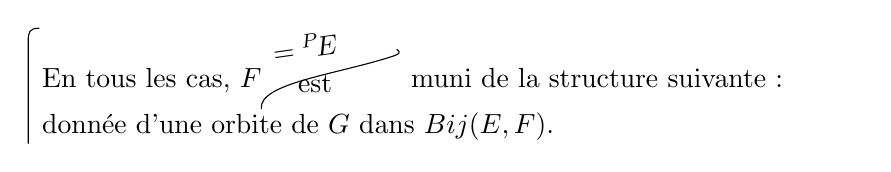
\begin{tikzpicture}[baseline=(body.north),x=1cm,y=1cm]
\node[anchor=north west,inner sep=0pt,text width=.86\linewidth] (body) at (0,0) {En tous les cas, \tikz[baseline=(f.base)]{
\node[anchor=base west,inner sep=0pt] (f) at (0,0) {$F$};
\node[anchor=base west,inner sep=0pt,rotate=8] at (.44,.32) {\inserted{$={}^{P}\!E$}};
\node[anchor=base west,inner sep=0pt] at (.74,-.06) {est};
\draw (.28,-.27) .. controls (.24,.06) and (1.25,.17) .. (1.95,.40)
 .. controls (2.03,.43) and (2.06,.44) .. (2.00,.49);
} muni de la structure suivante : donnée d'une orbite de $G$ dans $\operatorname{Bij}(E,F)$.};
% The main left boundary has a short upper hook and an open lower end.
\draw ([xshift=-.03cm,yshift=.02cm]body.north west)
 .. controls +(-.13cm,0) and +(0,.12cm) .. ([xshift=-.17cm,yshift=-.15cm]body.north west)
 -- ([xshift=-.17cm,yshift=-.04cm]body.south west);
\end{tikzpicture}

% The small bracketed note and the larger lowest line overlap on the sheet.
\noindent\hspace*{.29\linewidth}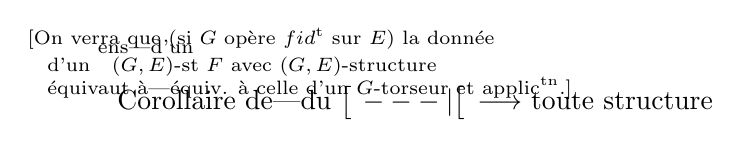
\begin{tikzpicture}[x=1cm,y=1cm,baseline=(smallone.base)]
\node[anchor=base west,inner sep=0pt,font=\scriptsize] (smallone) at (0,.46) {[On verra que (si $G$ opère $\unsure{\text{fid}^{\mathrm{t}}}$ sur $E$) la donnée};
\node[anchor=base west,inner sep=0pt,font=\scriptsize] at (.25,.12) {d'un \tikz[baseline=(old.base)]{
\node[anchor=base west,inner sep=0pt] (old) at (0,0) {\deleted{\unsure{$(G,E)$-st}}};
\node[anchor=base west,inner sep=0pt] at (-.18,.22) {\deleted{\unsure{ens|d'un}}};
} $F$ avec $(G,E)$-structure};
\node[anchor=base west,inner sep=0pt,font=\scriptsize] at (.25,-.17) {\unsure{équivaut à|équiv. à} celle d'un \unsure{$G$-torseur} \unsure{et applic$^{\mathrm{tn}}$}.]};
\node[anchor=base west,inner sep=0pt] at (1.14,-.37) {\uline{Corollaire} \unsure{de|du} $\unsure{\big[\,\mathbin{\text{---}}|\big[\,\longrightarrow}$ \unsure{toute structure}};
\end{tikzpicture}
% archive sheet number: 15
